% !TEX TS-program = pdflatex
% !TEX encoding = UTF-8 Unicode

% TeX-M (r1.1)
% For my math classes at UT Austin
% Notes template created by Abdon Morales for the College of Natural Science
% and for the Department of Mathematics and Computer Science
% (c) 2019 - 2024 Abdon Morales and the University of Texas at Austin
% This is a notes template for a LaTeX document using the "article" class for Mathematics (Calculus)
% at the University of Texas at Austin.

% Last change made: Jan 27, 2024 1:40 AM CST

% See "book", "report", "letter" for other types of document.

\documentclass[11pt]{article} % use larger type; default would be 10pt

% Start of Article customization options and addons (for more help and information reference to Overleaf's guides and docs on Latex.
\usepackage[utf8]{inputenc} % set input encoding (not needed with XeLaTeX)

%%% Examples of Article customizations
% These packages are optional, depending whether you want the features they provide.
% See the LaTeX Companion or other references for full information.

%%% PAGE DIMENSIONS
\usepackage{geometry} % to change the page dimensions
\geometry{letterpaper} % or letterpaper (US) or a5paper or....
% \geometry{margin=2in} % for example, change the margins to 2 inches all round
% \geometry{landscape} % set up the page for landscape
%   read geometry.pdf for detailed page layout information

\usepackage{graphicx} % support the \includegraphics command and options
\usepackage{xcolor}

% \usepackage[parfill]{parskip} % Activate to begin paragraphs with an empty line rather than an indent

%%% PACKAGES
\usepackage{booktabs} % for much better looking tables
\usepackage{array} % for better arrays (eg matrices) in maths
\usepackage{paralist} % very flexible & customisable lists (eg. enumerate/itemize, etc.)
\usepackage{verbatim} % adds environment for commenting out blocks of text & for better verbatim
\usepackage{subfig} % make it possible to include more than one captioned figure/table in a single float
\usepackage{exercise}
% Math tools
\usepackage{mathtools}
\usepackage{amsmath}
\usepackage{tikz} % For charts, mathematical graphs, and etc
%% Equal symbol for L'Hospital Rule
\usepackage{tcolorbox}
\newcommand\LR{\stackrel{\mathclap{\normalfont\mbox{L.R}}}{=}}
% These packages are all incorporated in the memoir class to one degree or another...

%%% HEADERS & FOOTERS
\usepackage{fancyhdr} % This should be set AFTER setting up the page geometry
\pagestyle{fancy} % options: empty , plain , fancy
\renewcommand{\headrulewidth}{0pt} % customise the layout...
\lhead{}\chead{}\rhead{}
\lfoot{}\cfoot{\thepage}\rfoot{}

%%% SECTION TITLE APPEARANCE
\usepackage{sectsty}
\allsectionsfont{\sffamily\mdseries\upshape} % (See the fntguide.pdf for font help)
% (This matches ConTeXt defaults)

%%% ToC (table of contents) APPEARANCE
\usepackage[nottoc,notlof,notlot]{tocbibind} % Put the bibliography in the ToC
\usepackage[titles,subfigure]{tocloft} % Alter the style of the Table of Contents
\renewcommand{\cftsecfont}{\rmfamily\mdseries\upshape}
\renewcommand{\cftsecpagefont}{\rmfamily\mdseries\upshape} % No bold!
%%% END Article customizations

%%% The "real" document content comes below...

% Replace examples with the actual content you intend to put
\title{Money and the Federal Reserve \\ Introduction to Macroeconomics}
\author{Abdon Morales \\ The University of Texas at Austin \\ ECO 304L \\ Wayne Geerling}
\date{\today \\ Chapter 17 : Week 11}
%\date{} % Activate to display a given date or no date (if empty),
         % otherwise the current date is printed 

\begin{document}
\maketitle
\subsection*{Controlling the money supply is not easy as you think}
Many people believe that managing the money we use in the economy is simple. After all, there's a fixed amount of paper currency and coins in circulation, and only the government has the authority to print more; but actually, creating more money isn't securely under the government's control as the printing-press model suggests. In fact, individuals and banks, not just in the United States but all around the world, have a hand in determining how many U.S dollars are coursing around the world economy.

What we use for "money" isn't always paper currency or coins; just think about your own daily purchases. Most, if not all, of them are paid for with something other than actual cash, right? The prices may be posted in dollars, but you might often pay with a debit card, a mobile payment app, or occasionally a personal check.

With a range of options that can be used in purchases, people have a lot more buying power than what's represented by physical currency. This makes it hard to get an exact fix on the size of the money supply.

The last two chapters focused on government budgets and fiscal policy; in this chapter and the next, we turn to the second major category of macroeconomic policy: monetary policy. We begin by looking closely at the definition of money - its functions and its different forms; because banks play an integral role in the money supply process, we discuss how they operate, and how their decisions affect the amount of money in the economy. Finally, we look at the role of the Federal Reserve System and examine how it oversees our monetary system and the health of our economy. This background provides essential preparation for further discussion of monetary policy in Chapter 18.

\begin{tcolorbox}[width=\textwidth,colback={white},title={Big Questions},colbacktitle=yellow,coltitle=blue]
\begin{itemize}
\item What is money?
\begin{itemize}
\item Money is primarily the medium of exchange in an economy; it's what people trade for goods and services. Money also functions as a unit of account and a store of value.
\item Money includes more than just physical currency; it also includes bank deposits because people often make purchases with checks or cards that withdraw from their bank accounts.
\end{itemize}
\item How do banks create money?
\begin{itemize}
\item Banks create money whenever they extend a loan. A new loan represents new purchasing power, while the deposit that backs the loan is also considered money.
\end{itemize}
\item How does the Federal Reserve implement monetary policy?
\begin{itemize}
\item The Fed has several other tools it can use to control the money supply, including interest paid on bank reserves, open market operations, the discount window and other lending facilities, and the discount rate.
\end{itemize}
\end{itemize}
\end{tcolorbox}

\section*{\textbf{What is money?}}
What is money? The question may seem odd...after all, we use money all the time, right? Even children know that we use coins and paper bills to buy things; those coins and constitute \textbf{\textcolor{red}{currency}}, but people also make many purchases without currency. Our definition of \textit{money} is much broader: \textbf{\textcolor{red}{money}} is any generally accepted means of payment. In this section, we define the functions of money and the explain how the quantity of money is measured.

\subsection*{\textbf{\textit{Three functions of money}}}
Money has three functions: it is a medium of exchange, a unit of account, and a store of value. Let's look at each function.
\subsubsection*{\textcolor{olive}{A medium of exchange}}
\subparagraph*{
If you want to buy groceries, you offer money in exchange for them; if you work, you accept money as payment for your labor. Money is a common \textbf{\textcolor{red}{medium of exchange}} - that is, it is what people trade for goods and services.
}
\subparagraph*{
Modern economies generally have a government-provided medium of exchange. In the United States, the government provides our dollar currency; but even in economies without government provision, a preferred medium of exchange usually emerges.
}
\subparagraph*{
Invariably, some medium of exchange evolves in any economy; the primary reason is the inefficiency of barter, which is money's alternative. \textbf{\textcolor{red}{Barter}} occurs when there is no commonly accepted medium of exchange; it involves individuals trading some good or service they already have for something else they want. Barter requires a \textbf{\textcolor{red}{double coincidence of wants}}, in which each party in an exchange transaction happens to have what the other party desires. A double coincidence is pretty unusual, which is why a medium of exchange naturally evolves in any exchange environment.
Historically, the first medium of exchange in an economy has been a commodity used to trade for goods and services. \textbf{\textcolor{red}{Commodity money}} involves the use of an actual good for money; in this situation, the good itself has value apart from its function as money. Money typically evolves into certificates that represent a fixed quantity of the commodity; these certificates become the medium of exchange but are still tied to the commodity, because they can be traded for the actual commodity if the holder demands it.
}
\subparagraph*{
\textbf{\textcolor{red}{Commodity-backed money}} is money you can exchange for a commodity at a fixed rate. For example, until 1971, U.S dollars were fixed in value to specific quantities of silver and gold. A \$1 U.S silver certificate looks much like dollar bills in circulation today, but the print along the bottom of the note reads, "One dollar in silver payable to the bearer on demand." Until 1964, we also had commodity coins in the United States.
}
\subparagraph*{
While commodity money and commodity-backed money evolves privately in all economies, the type of money used in most modern economies depends on government. In particular, most modern economies make use of fiat money for their medium of exchange; \textbf{\textcolor{red}{Fiat money}} is money with no value except as the medium of exchange, there's no inherent or intrinsic value of the currency. In the United States, our fiat currency is physically just pieces of green paper, otherwise known as Federal Reserve Notes; this paper has value because the government has mandated that we can use the currency to pay our debts [On U.S dollars bills, you can read the statement "This note is legal tender for all debts, public and private."].
}
\subparagraph*{
There are advantages and disadvantages to fiat and commodity monies. On the one hand, commodity-backed money ties the value of the holder's money to something real; if the government is obligated to trade silver for every dollar in circulation, this limits the number of dollars the government can print, which keeps a lid of inflation. Fiat money offers no such constraint on the expansion of the money supply; rapid monetary expansion and then inflation can occur without a commodity standard that ties the value of money to something real.
}
\subparagraph*{
On the other hand, tying the value of a nation's currency to a commodity is dangerous when the market value of the commodity fluctuates. Imagine how a new discovery of gold affects prices in a nation with gold-backed currency; an increased supply of gold reduces gold prices, and therefore more gold is required in exchange for all other goods and services. This inflation: the price of everything in terms of money (gold) rises. Because a change in the value of a medium of exchange affects the prices of all goods and services in the macroeconomy, it can be risky to tie a currency to a commodity.
}

\subsubsection*{\textcolor{olive}{A unit of account}}
\subparagraph*{
Money also serves as a unit of account; a \textbf{\textcolor{red}{unit of account}} is the measure in which prices are quoted. Money enables you and someone you don't know to speak a common language.
}
\subparagraph*{
Expressing the value of something in terms of dollars and cents also enables people to make accurate comparisons between items. Thus, money also serves as measuring stick and recording device; in everyday conversation, we use dollars to measure relative values. How much is your backpack or cell phone worth, or your computer? Your answer is in dollars and cents; you use dollar amounts to keep track of your bank account and to record transactions in a consistent manner.
}
\subsubsection*{A store of value}
\subparagraph*{Money's third function is as a store of value. A \textbf{\textcolor{red}{store of value}} is a means for holding wealth; money has long served as an important store of value. Today, we have other options for holding our wealth, many of which offer greater returns than keeping dollar bills in a sock drawer or stuffed under a mattress. We can easily put our dollars into bank accounts or investment accounts that earn interest; these options have caused money's role as a store of value to decline.}

\subsection*{Measuring the quantity of money}
Now that we have defined the three functions of money, we need to consider how the total amount of money in the economy is measured. As we saw in Chapter 8, the quantity of money in an economy affects the overall price level. In particular, a nation's inflation rate is dependent on the rate of growth of its quantity of money, in addition, in Chapter 18 we'll see that the quantity of money can influence real GDP and unemployment rates because money has such profound macroeconomics influences. You might think it is important to measure it accurately; unfortunately, this is not the cause as easy as it once was.

To measure the quantity of money in an economy, we must somehow find the total value of all these alternatives means people to use to buy goods and services. Clearly, currency alone is not enough - people buy things all the time without using currency. Currency is money, but it constitutes only a small part of the total money supply.

Because it is so hard these days to measure the overall amount of money in circulation, the Fed closely monitors interest rates, like the federal funds rate (which we will talk about). Interest rates are the prices of funds in the banking system, so they help the Fed gauge whether there is too little or too much money in the economy. These give an indication of the overall amount of money circulating in the banking system.
\subsubsection*{\textcolor{olive}{M1 and M2}}
\subparagraph*{As we broaden our definition of money beyond currency, we first acknowledge bank deposits on which checks can be written; \textbf{\textcolor{red}{checkable deposits}} are deposits in bank accounts from which depositors may make withdrawals by writing checks. These deposits represent purchasing power very similar to currency, because many sellers accept personal checks; savings deposits are another large category of deposits that count when we measure the money supply, since we easily access these via ATMs or debit cards. Adding checkable deposits and savings deposits to currency gives us a money supply measure known as \textbf{\textcolor{red}{M1}}.}
\subparagraph*{At one time, savings deposits were excluded from M1 but included in broader money supply measure called \textbf{\textcolor{red}{M2}}. Starting in May 2020, however, savings deposits became part of M1, and so M2 and M2 are now almost identical; the only difference is that M2 adds two minor components: small time deposits and retail money market funds.}
\subparagraph*{The key point to remember is that the money supply in an economy includes both currency and bank deposits; note that credit cards are not part of the money supply. Purchases made with credit cards involve a loan extended right at the cash register; when the loan is made, a third party is paying for the purchase until the loan is repaid. Because credit cards purchases involve the use of borrowed funds, credit cards are not included as part of the money supply.}
\begin{center}
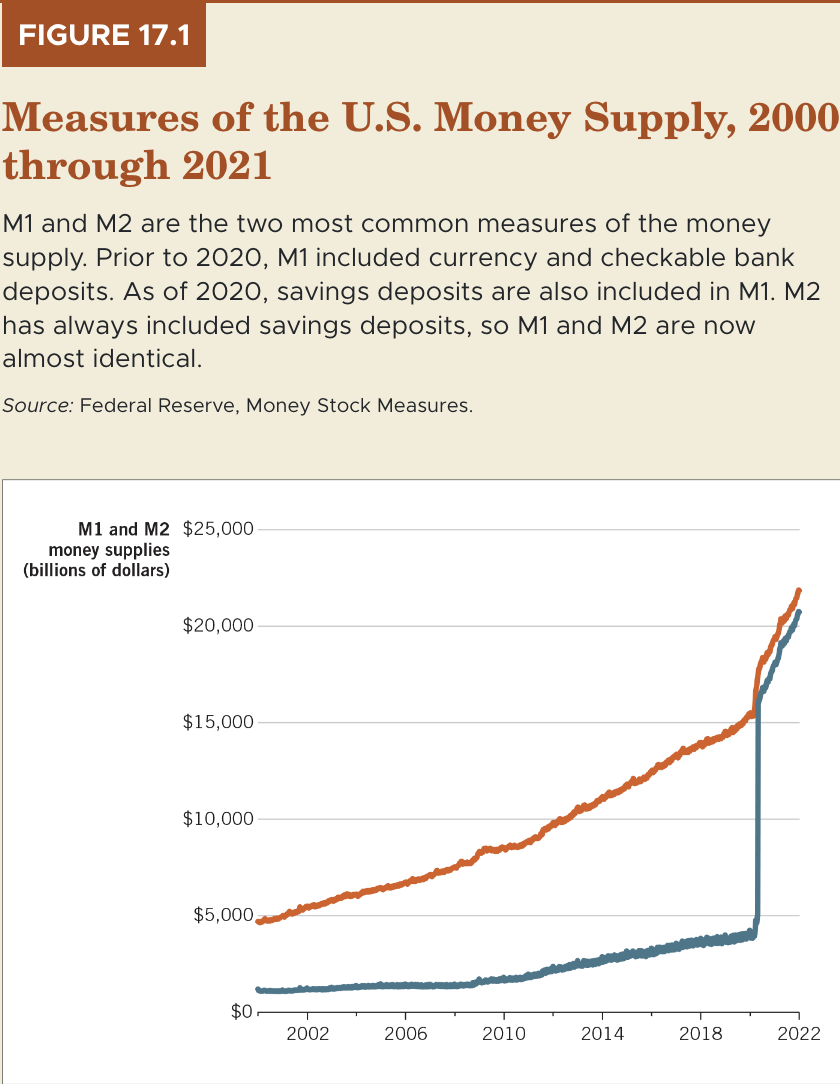
\includegraphics[scale=0.5]{../../Chapter 17 Money and the Federal Reserve/Notes/images/Figure 17.1.png} 
\end{center}

\section*{How do banks create money?}
We now have a working definition of money: money includes both currency and deposits at banks; and while private individuals and firms aren't permitted to print currency, private actions do influence the supply of money in the economy, because both private individuals and banks affect deposits. In this section, we explain how banks create money as a by-product of their daily business activity. Note that when we refer to "banks", we are talking about commercial banks, which take in deposits and extended loans. We distinguish commercial banks from investment banks, which serve a different role.

We begin by looking closely at daily activities at typical banks. After that, we consider how banks influence the money supply.

\subsection*{The Business of Banking}
Banks serve two very important roles in the macroeconomy; first, they are middlemen in the market for loanable funds. As we saw in Chapter 10, they provide a way for savers to supply their funds to borrowers without purchasing a financial security. Second, they play a role in creating the supply of money.

To understand how banks create money, let us consider the functions of a bank, illustrated in Figure 17.2; banks are go-betweens in the markets for loans. They are financial intermediaries; that is, they take in deposits and extend loan. Deposits are the primary source of funds, and loans are the primary use of these funds. Banks can be profitable if the interest rate they charge on loans is higher than the interest rate they pay out on deposits.
\begin{center}
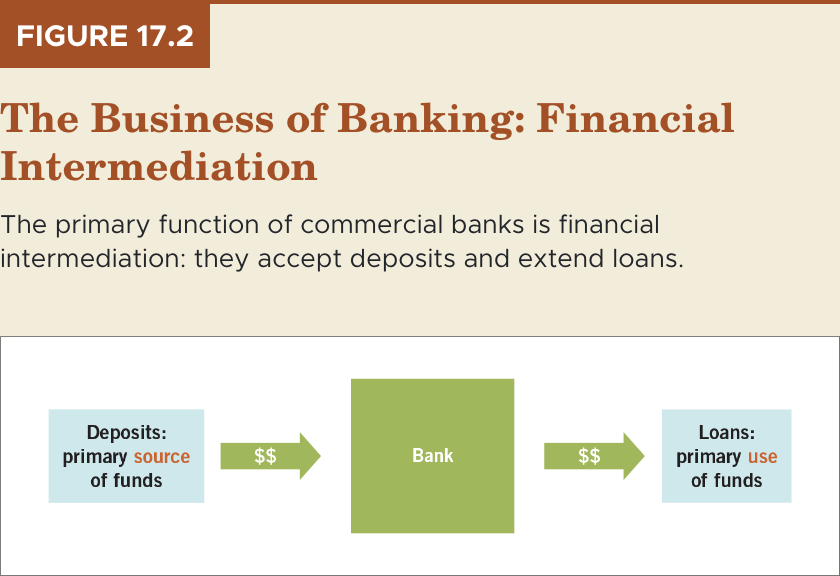
\includegraphics[scale=0.5]{../../Chapter 17 Money and the Federal Reserve/Notes/images/Figure 17.2.png}
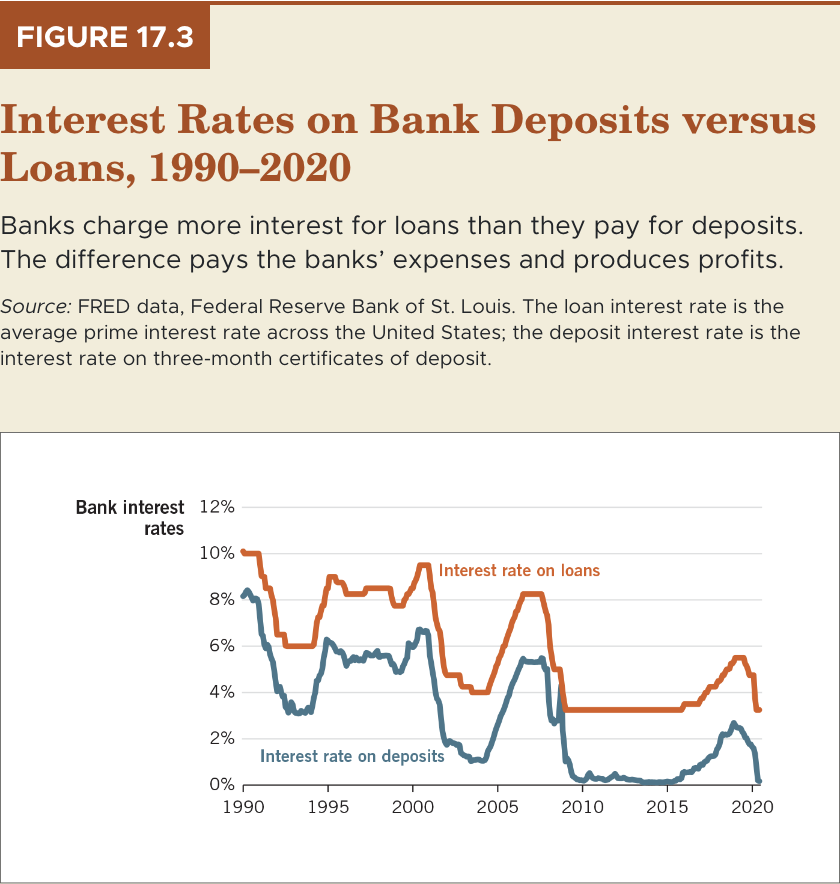
\includegraphics[scale=0.5]{images/Figure 17.3.png} 
\end{center}

\subsubsection*{\textcolor{olive}{The bank's balance sheet}}
\subparagraph*{Information about a bank's financial operations is available in the bank's balance sheet. A \textbf{\textcolor{red}{balance sheet}} is an accounting statement that summarizes a firm's key financial information. The left side of the balance sheet details the bank's \textbf{\textcolor{red}{assets}}, which are the items that the firm owns. Assets indicate how the banking firm uses the funds it has raised from various sources; the right side of the balance sheet details the bank's liabilities and owner's equity. \textbf{\textcolor{red}{Liabilities}} are the financial obligations the firm owes to others; \textbf{\textcolor{red}{Owner's equity}} (sometimes called \textit{\textbf{shareholders' equity}}) is the difference between the firm's assets and its liabilities. When a firm has more assets than liabilities, it has positive owner's equity; overall, the right side of the balance sheet identifies the bank's sources of funds.}
\begin{center}
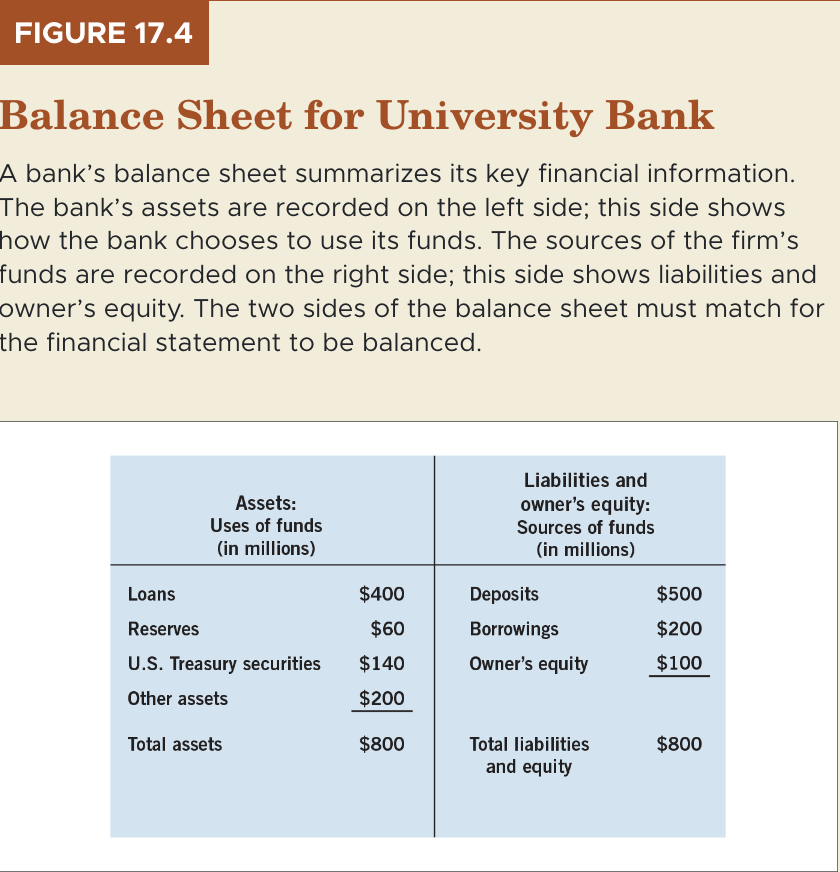
\includegraphics[scale=0.5]{images/Figure 17.4.png} 
\end{center}
\subparagraph*{\textbf{\textcolor{red}{Reserves}} are the portion of bank deposits set aside and not loaned out. Reserves include both currency in the bank's vault and funds that the bank holds in deposit at its own bank, the Federal Reserve; banks also hold U.S Treasury securities and other government securities as substantial assets in their portfolio. These securities earn interest and carry very low risk. Finally, banks hold other assets, such as physical buildings and furniture.}
\subparagraph*{The right side of the balance sheet displays the major sources of funds for banks. Banks fund their activities primarily by taking in deposits; in fact, the deposits of typical households are the lifeblood of banks. Banks also borrow from other commercial banks and from the Federal Reserve. \\In the next section, we look more closely at bank reserves, which play an important role in money creation.}

\subsubsection*{\textbf{\textcolor{olive}{Bank reserves}}}
\subparagraph*{Our modern system of banking is a fractional reserve system; \textbf{\textcolor{red}{Fractional reserve banking}} occurs when banks hold only a fraction of deposits on reserve.\\Still, banks do hold more deposits on reserve in order to accommodate withdrawals by their depositors. You'd be pretty unhappy if you tried to make a withdrawal from your bank and it didn't have enough on reserve to honor your request. If word spread that a bank might have difficulty meeting its depositors' withdrawal requests, it might lead to a bank run. A \textbf{\textcolor{red}{bank run}} occurs when many depositors attempt to withdraw their funds from a bank at the same time.}
\subparagraph*{Before 2020, banks were required to hold a certain portion of their deposits in reserve; the required fraction was called the required reserve ration. \textit{For a given bank, the dollar amount of required reserves was required determined by multiplying the required reserve ration by the bank's total amount of deposits.}}

\begin{center}
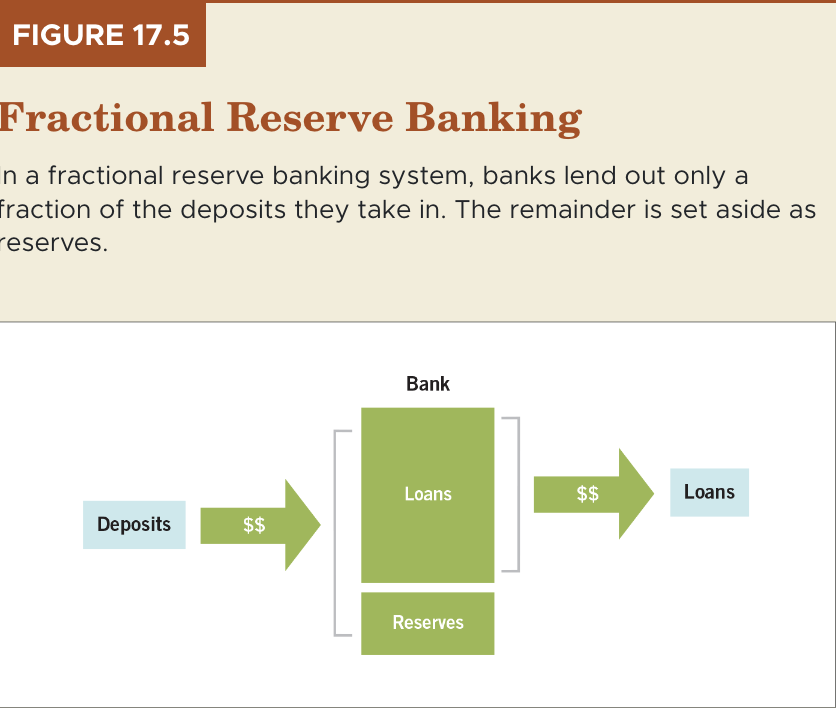
\includegraphics[scale=0.5]{images/Figure 17.5.png} 
\end{center}

\subsubsection*{\textcolor{olive}{The FDIC and Moral Hazard}}
\subparagraph*{Because a bank keeps only a fraction of its deposits on reserve, if all depositors try to withdraw their deposits at the same time, the bank will not be able to meet its obligations. But in a typical fay, only a small number of deposits are withdrawn; in the past, when word spread that a bank was unstable and perhaps could not meet the demand of depositors - whether this rumor was true or not - depositors would rush to with draw their funds, leading to a bank run.}
\subparagraph*{After the massive rate of bank failures from 1929 to 1933, the U.S government instituted federal deposit insurance in 1933 through the Federal Deposit Insurance Corporation (FDIC). Deposit insurance now guarantees that depositors will get their deposits back (up to \$250,000) even if their bank goes bankrupt. FDIC insurance greatly decreased the frequency of bank runs; unfortunately, deposit insurance also created what we call a moral hazard situation. \textbf{\textcolor{red}{Moral hazard}} is the lack of incentive to guard against risk where one is protected from its consequences. FDIC insurance means that neither banks nor their depositors have an incentive to monitor risk; no matter what happens, they're protected from the consequences of risky behavior.}
\subparagraph*{There is a tremendous upside and no significant downside, because depositors are protected against losses by FDIC insurance. This is the environment in which modern banks operate, which is why many analysts argue that reserve requirements and other regulations are necessary to help ensure stability in the financial industry - especially given the recessions often start in the financial industry.}
\subsection*{\textbf{Creating money by multiplying deposits}}
We have seen that banks function as financial intermediates; but as a by-product of their everyday activity, they also create new money. Modern U.S banks don't mint currency, but they do create new deposits, and deposits are a part of the money supply.

This is just the first step in the money creation process; we'll now explore this process in more detail, utilizing the bank's balance sheet. For this example, we make two simplifying assumptions to help understand the general picture:\\
\begin{center}
\noindent\begin{minipage}{\linewidth}
\centering
Assumption 1: All currency is deposited to banks\\
Assumption 2: All banks decide to keep 10\% of deposits on reserve
\end{minipage}
\end{center}
In the end, the impact on the money supply is a large multiple of the initial increase in money; the exact multiple depends on the \textbf{\textcolor{red}{reserve ration}}(rr) the banks decide to maintain. The rate at which banks multiply money when all currency is deposited into banks (Assumption 1) is called the \textbf{\textcolor{red}{simple money multiplier}}$(m^m)$. The formula for the simple money multiplier is:
\begin{center}
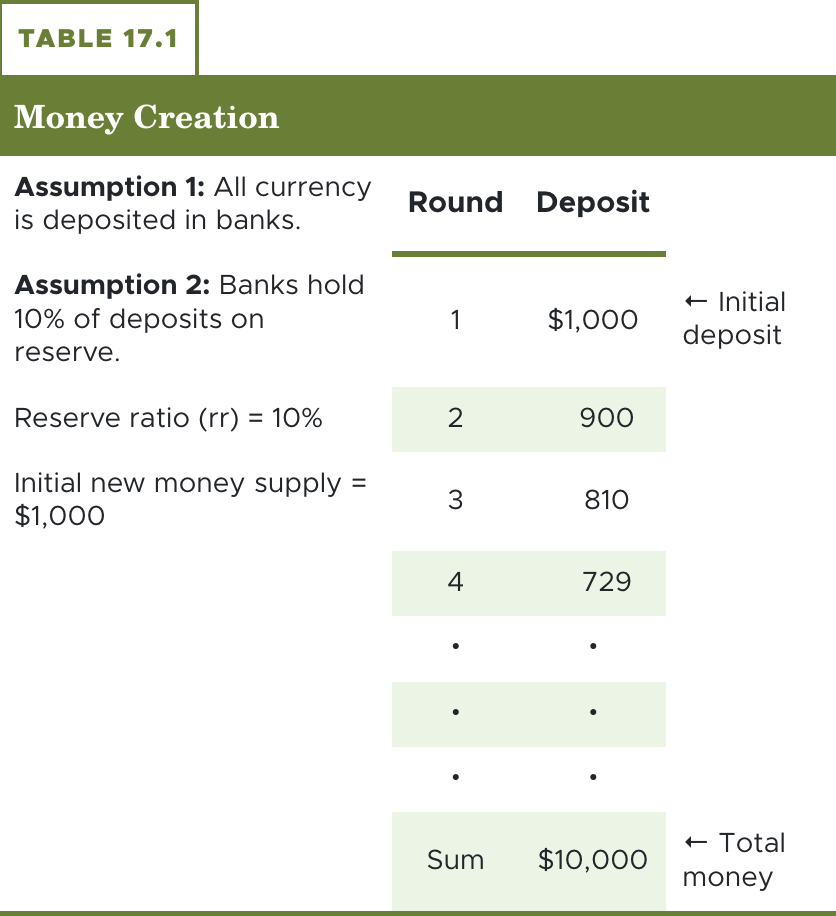
\includegraphics[scale=0.5]{images/Table 17.1.png}
\begin{equation}
m^m = \frac{1}{rr}
\end{equation}
\end{center}
In our example [to added here, reference the textbook], rr = 0.10, so the multiplier is $\frac{1}{0.10}$, which is 10. When the money multiplier is 10, a new \$1,000 bill produced by the Federal Reserve can eventually lead to \$10,000 in new money.

Of course, in the real world our two assumptions don't always hold. There is a more realistic money multiplier that relaxes the two assumptions; consider how a real-world money multiplier would compare with the simple money multiplier. First, if people hold on to some currency (relaxing Assumption 1), banks cannot multiply that currency, so the more realistic multiplier is smaller than the simple money multiplier. On the other hand, when banks hold less on reserve (relaxing Assumption 2), more dollars are multiplied, and the real multiplier is larger than the simple version.

Note that the money multiplier process also works in reverse; when funds are withdrawn from the banking system, these are funds that banks cannot multiply. In effect, the money supply contracts.

\section*{How does the federal reserve implement monetary policy?}
There's a good chance you've heard of the U.S Federal Reserve (Fed), even outside economics class. Jerome Powell, the current Chair of the Fed's Board of Governors, is one of the most recognized economic policymakers in the world; and while we've referred to the Fed periodically throughout this text, how it's time to examine it closely.

\subsection*{The many jobs of the Federal Reserve}
The Fed was established in 1913 as the central bank of the United States; the Fed's primary responsibilities are threefold:
\begin{enumerate}
\item \textit{\textbf{Monetary policy}}: The Fed is charged with managing monetary policy so as to promote maximum employment and stable prices effectively.
\item \textit{\textbf{Central banking}}: The Fed serves as a bank for banks, holding their deposits and extending loans to them.
\item \textit{\textbf{Bank regulation}}: The Fed is one of the primary entities charged with ensuring the financial stability of banks.
\end{enumerate} 
In this section, we talk about the Fed's role as central bank and bank regulator. We then look at monetary policy in the remainder of the chapter and into the next chapter.

The Fed is a "central bank" - that is, it acts as a "bank for banks." In its role as central bank, it offers support and stability to the nation's entire banking system; the first component of this role involves the deposits that banks hold at the Fed. \textbf{\textcolor{red}{Federal funds}} are deposits that private banks hold on reserve at the Fed, and, as of 2008, the Fed pays interest on these deposits. The word "federal" seems to denote that the deposits are government funds, but in fact they are private funds held on deposit at a \textit{\textbf{federal agency}} - the Fed. These deposits are part of the reserves that banks set aside, along with the physical currency in their vaults.

Banks keep reserves at the Fed in part because the Fed clears loans between banks. When banks loan reserves to other banks, these are \textit{\textbf{federal funds loans}}. The federal funds loans are typically very short term (often overnight), and they enable banks to make quick adjustments to their balance sheets. The interest rate that banks charge each other on interbank loans is known as the \textbf{\textcolor{red}{federal funds rate}}. This rate moves up and down based on the borrowing and lending choices of individual banks; the federal funds rate is generally higher than the interest rate banks earn on their reserves at the Fed.

The federal funds rate is one of the most closely monitored interest rates in the world. This is the interest rate that the Fed "targets", for monetary policy; because the actual quantity of money in the economy is hard to measure, the Fed monitors conditions in the banking system by watching the federal funds rate (among other indicators). In the next section, we'll discuss how the Fed acts to push the federal funds rate up and down, depending on macroeconomic conditions.
\begin{center}
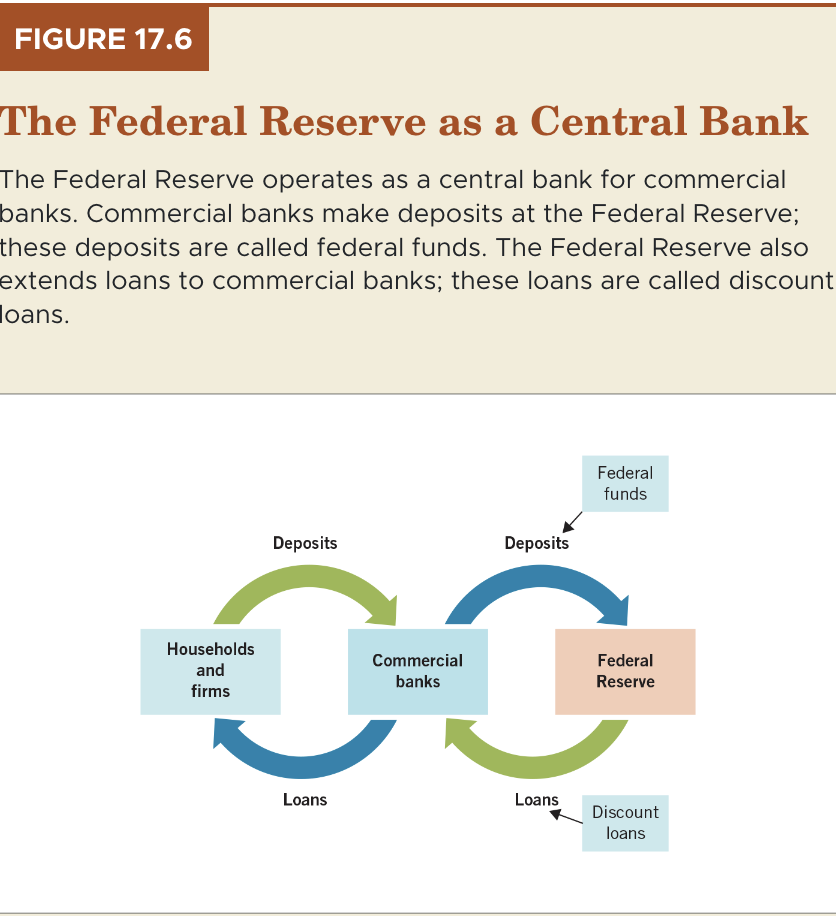
\includegraphics[scale=0.5]{images/Figure 17.6.png} 
\end{center}

Figure 17.6 illustrates how the relationship between the Federal Reserve and commercial banks is analogous to the relationship between commercial banks and households and firms. First, households and firms hold deposits at banks, and banks hold deposits at the Fed - these are the federal funds; second, households and firms take out loans from banks, and banks take out loans from the Fed. The loans from the Fed to private banks are known as \textbf{discount loans}.

Discount loans are the vehicle by which the Fed performs its role as "lender of last resort". Given the macroeconomic danger of bank failure, the Fed serves an important role as a backup lender to private banks that find difficulty borrowing elsewhere. The \textbf{\textcolor{red}{discount rate}} is the interest rate on the discount loans made from the Fed to private banks. The Fed sets this interest rate because it is a loan directly from a branch of the U.S government to private financial institutions.

Discount loans don't often figure prominently in macroeconomics, but in extremely turbulent times, they reassure financial market participants.

The Fed also serves as a regulator of individual banks; the Fed monitors the balance sheets of banks with an eye toward limiting the riskiness of the assets the banks hold. One might ask why banks are subject to this kind of regulation; after all, the government doesn't monitor the riskiness of assets owned by other private firms. However, as we have seen, the interdependent nature of banking firms means that banking problems often spread throughout the entire industry very quickly. In addition, there is the moral hazard problem we discussed earlier: because of deposit insurance, banks, and their customers have reduced incentives to monitor the risk of bank assets on their own.

\subsection*{Monetary Policy Tools}
The Federal Reserve has been actively managing the money supply for over a century; but the last two recessions have changed the way the Fed reacts in times of crisis. In addition, because the money supply is difficult to measure, the Fed generally watches market indicators like the federal funds rate to determine the correct stance for monetary policy.

In this section, we discuss the tools the Fed used to affect the economy, with emphasis on the primary tools used to combat recent recessions. We begin with a relatively new tool, the interest rate paid on bank reserves.

\subsubsection*{\textcolor{olive}{Interest rate on bank reserves}}
\subparagraph*{Prior to 2008, bank reserves earned no interest; in that era, there were real opportunity costs to holding reserves, because banks could earn interest on loans or by buying financial securities. But in October 2008, the Federal Reserve began paying interest on bank reserves; The rate of interest, known as the \textbf{\textcolor{{red}{interest on reserve balance (IORB)}}, is known an important policy tool. Immediately, banks start holding more reserves.
}
\subparagraph*{
A reduction in the IORB leads banks to make additional loans, which increases the money supply. This tool can also work in reverse: if the Fed wishes to pull back, it can raise the IORB, causing banks to hold onto more reserves, which dampens the money multiplication process.
}
\subparagraph*{
The power of this new tool is still open to debate; as of 2022, banks still held on to significant reserves, even after the interest rate had dropped back down to just 0.15\%.
}
\begin{center}
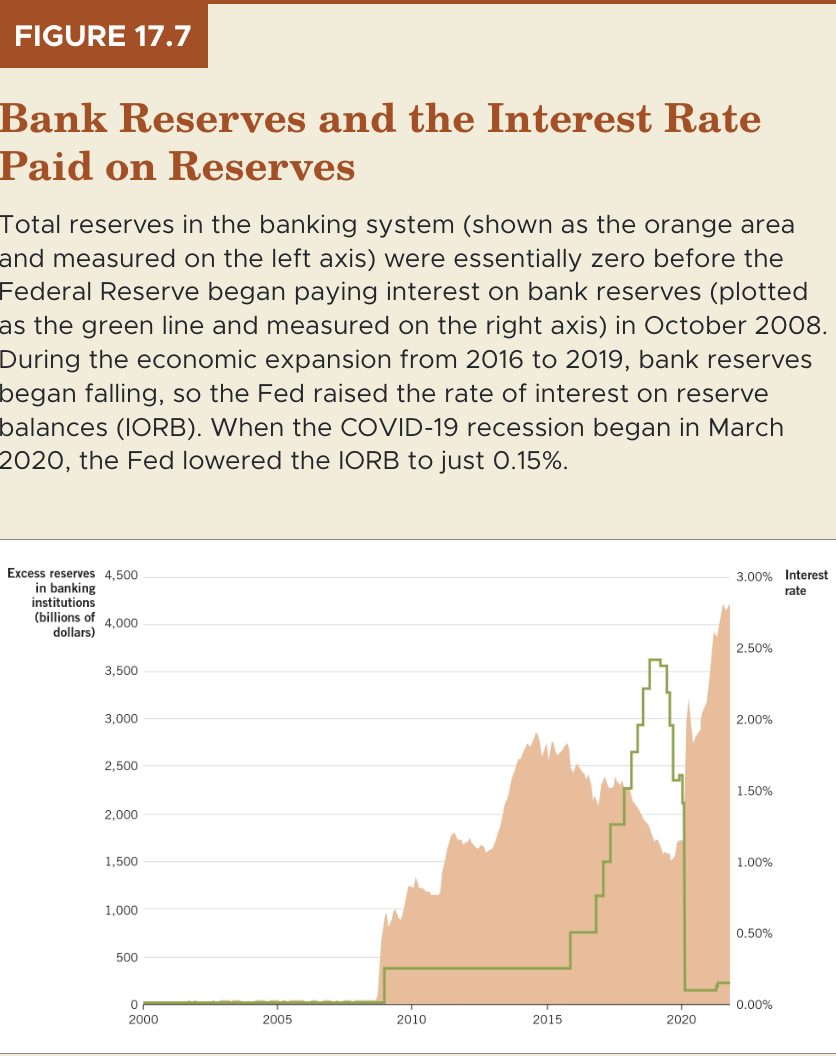
\includegraphics[scale=0.5]{images/Figure 17.7.png} 
\end{center}
\subsubsection*{\textcolor{olive}{Open Market Operations}}
\subparagraph*{The Fed can also insert money directly into the economy.}
\subparagraph*{\textbf{\textcolor{red}{Open market operations}} involve the purchase or sale of bonds by central bank. When the Fed wants to increase the money supply, it buys securities; in contrast, when it wishes to decrease the money supply, it sells securities. In Chapter 10, we introduced the U.S Treasury security as a special bond asset. Normal or "traditional" open market operations involve buying and selling short-term (less than one year) Treasury securities.}
\subparagraph*{There are at least two good reasons why the Fed chooses the Treasury security market for open market operations. First, the Fed's goal is to get funds directly into the market for loanable funds, in this way, financial institutions begin lending the new money, and it quickly moves into the economy. Second, a typical day's worth of open market operations might entail as much as \$20 billion in purchases.}
\subparagraph*{When the Fed buys Treasury securities held by financial institutions (panel[a]), the Fed pays for those bonds using money it creates. The result is more money circulating in the economy, and this shows up as a reduction in the federal funds rate. On the flip side, when the Fed sells bonds to financial institutions (panel[b]), the money it receives in exchange is taken out of the economy, leaving less money in circulation and a higher federal funds rate. In reality, the Fed undertakes open market operations every business day; typically, it aims to keep market conditions exactly as they were the day before, but the Fed also uses open market operations to increase the money supply to offset recessions.}
\begin{center}
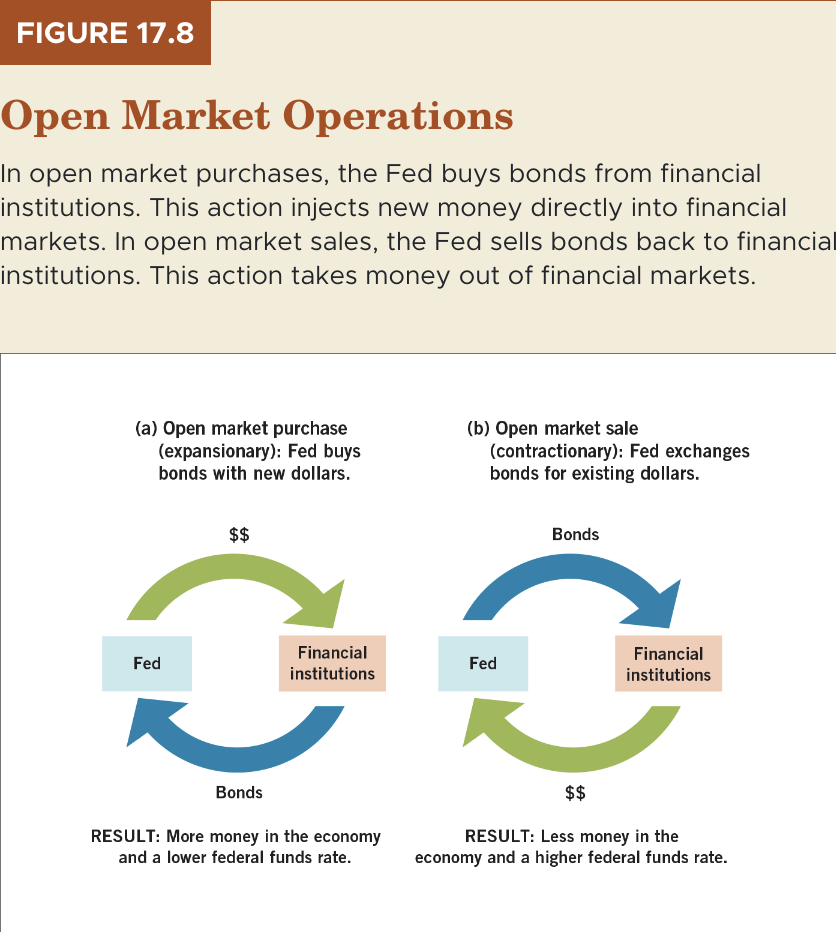
\includegraphics[scale=0.5]{images/Figure 17.8.png} 
\end{center}
\subparagraph*{Open market operations typically involve buying and selling short-term Treasury securities - that is, bonds that mature in less than a year. In \textbf{\textcolor{red}{quantitative easing}}, the central bank buys longer-term Treasury securities and other types of securities, specifically targeting certain markets. [During the Great Recession,] the Fed bought mortgage-backed securities that were considered "toxic assets", meaning assets loaded with risk that could destabilize private markets.
}

\subsubsection*{\textcolor{olive}{The discount window and new lending facilities}}
\subparagraph*{Earlier in this chapter, we discussed the Fed's \textbf{\textcolor{red}{discount window}}, as it's called, and the rate the private banks pay on these loans is known as the discount rate. In the past, the Fed would increase the discount rate to discourage borrowing by banks and to decrease the money supply, and it would decrease the discount rate to encourage borrowing by banks and to increase the money supply. These days, instead of being actively managed, the discount rate is generally pegged near the federal funds rate. However, the discount window is still a critical safety net for struggling banks.}
\subparagraph*{It also lends directly to private institutions; until recently, this was an extremely minor part of the Fed's overall involvement with the economy. However, direct Fed lending has expanded in both size and scope since the beginning of the Great Recession; this is the second major recent innovation in monetary policy (along with the active use of the IORB). To keep that from happening, the Fed began lending extensively to firms in those markets, through \textbf{\textcolor{red}{lending facilities}} set up for that purpose. These early lending facilities were, in effect, discount windows for private financial firms.}
\subsection*{\textcolor{olive}{Reserve Requirements}}
\subparagraph*{In the past, the Fed also made use of reserve requirements to administer monetary policy. In March 2020, however, the Fed announced that it would no longer require banks to set aside a portion of deposits on reserve. Historically, though, this was an important tool that the Fed used to affect the money multiplier, and it is still used by many other nations. When the Fed lowered the required reserve ratio, the money multiplier increased. When it raised the required reserve ration, the money multiplier fell.}
\subparagraph*{This tool was not as precise or predictable as open market operations because small changes in the money multiplier could lead to large swings in the money supply, changing the reserve requirement caused the money supply to change too much. In addition, changing reserve requirements also had unpredictable outcomes because the overall effects depended on the actions of banks. It was possible that the Fed would lower the reserve requirement to 5\% and banks would not change their reserves. For those reasons, the reserve requirement that had not been used for monetary policy since 1992. In addition, as part of the March 2020 response to the coronavirus crisis, the Fed completely eliminated reserve requirements, hoping this would get banks to lend aggressively.}
\begin{center}
Table 17.2 summarizes the Fed's monetary policy tools; the tools developed recently are highlighted in orange.\\
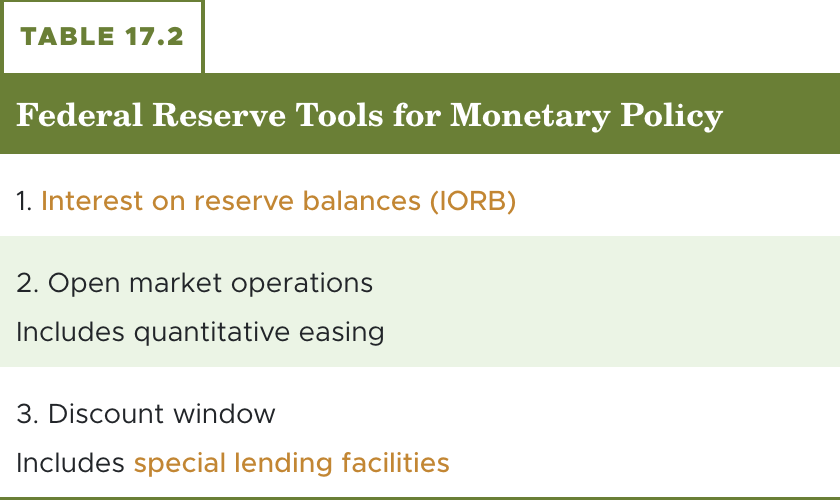
\includegraphics[scale=0.5]{images/Table 17.2.png} 
\end{center}

\section*{Conclusion}
We started this chapter with a common misconception about the supply of money in an economy. Many people believe that it is pretty simple to regulate the quantity of money in an economy; but while currency in modern economies is issued exclusively by government, money also includes bank deposits. Banks expand the money supply when they extend loans, and they contract the money supply when they increase their level of reserves. Even individuals have a significant influence: people like you and me cause the money supply to rise and fall when we change how much currency we hold outside the banking system. Taken together, these facts mean that the Fed's job of monitoring the quantity of money is very difficult; the Fed attempts to expand or contract the money supply, but its efforts may be offset by the actions of banks and individuals.

The material in this chapter sets the stage for a theoretical discussion of monetary policy and the way it affects the economy, which we undertake in the next chapter.
\end{document}